%%%%%%%%%%%%%%%%%%%%%%%%%%%%%%%%%%%%%%%%%%%%%%%%%%%%%%%%%%%%%%%%%%%%%%%%%%%%% 
%
% This is a LaTeX file for an A0 poster.
% 
% template poster taken from https://canizo.org/latex_poster
%
%%%%%%%%%%%%%%%%%%%%%%%%%%%%%%%%%%%%%%%%%%%%%%%%%%%%%%%%%%%%%%%%%%%%%%%%%%%%% 

%%%%%%%%%%%%%%%%%%%%%%%%%%%%%%%%%%%%%%%%%%%%%%%%%%%%%%%%%%%%%%%%%%%%%%%%%%%%% 
%%%%%%%%%%%%%%%%%%%%%%%%%%%%%%%%%%%%%%%%%%%%%%%%%%%%%%%%%%%%%%%%%%%%%%%%%%%%%
%
% scpdata: a data package for single-cell proteomics
%
% Poster for the Eurobioc2019, December 2019.
%
%%%%%%%%%%%%%%%%%%%%%%%%%%%%%%%%%%%%%%%%%%%%%%%%%%%%%%%%%%%%%%%%%%%%%%%%%%%%%
%%%%%%%%%%%%%%%%%%%%%%%%%%%%%%%%%%%%%%%%%%%%%%%%%%%%%%%%%%%%%%%%%%%%%%%%%%%%%

\documentclass{article}
% To modify the size of the page:
\usepackage[dvips,a3paper,portrait,centering,margin=0.4cm]{geometry}
% To create multiple columns
\usepackage{multicol}

\usepackage[utf8]{inputenc}
% To align images
\usepackage[export]{adjustbox}
% Use captions in minipages
\usepackage{caption}
% Math font
\usepackage{amsmath, amsthm, amsfonts}
% Include figure files.
\usepackage{graphicx}

% Coding fonts
% ------------
% For including R chunks 
\usepackage{listings} 
\lstset{
  language=R,
  basicstyle=\small\ttfamily\color{vdgray},       % the size of the fonts that are used for the code
  % sensitive=false,
  numbers=left,                   % where to put the line-numbers
  numberstyle=\tiny\color{gray},  % the style that is used for the line-numbers
  stepnumber=1,                   % the step between two line-numbers.
  numbersep=0.1cm,                % how far the line-numbers are from the code
  backgroundcolor=\color{lgray},  % choose the background color. You must add \usepackage{color}
  deletekeywords={stat},
  keywordstyle=\color{blue},      % keyword style
  stringstyle=\color{green},      % string literal style
  xleftmargin=0.5cm,
}
% Create command for highlighting inline code or variables
\newcommand{\hcode}[2][lgray]{{\ttfamily\color{vdgray}\colorbox{#1}{#2}}}

% Colors
% ------
\usepackage{color}
\usepackage[dvipsnames]{xcolor}
% Color panel used throughout the poster
\definecolor{lgray}{rgb}{0.9179688,0.9179688,0.9179688} % #ebebeb
\definecolor{dgray}{rgb}{0.796875,0.796875,0.796875} % #cccccc
\definecolor{vdgray}{rgb}{0.3984375,0.3984375,0.3984375} % #666666
\definecolor{coral}{rgb}{0.9960938,0.4960938,0.3125000} % #ff7f50
\definecolor{blue}{rgb}{0.4218750,0.6484375,0.8007812} % #6ca6cd
\definecolor{green}{rgb}{0.6992188,0.7265625,0.5078125} % #b3ba82
\definecolor{yellow}{rgb}{0.9570312,0.8671875,0.6992188} % #f5deb3

% Adjust space between reference items
% ------------------------------------
\let\OLDthebibliography\thebibliography
\renewcommand\thebibliography[1]{
  \OLDthebibliography{#1}
  \setlength{\parskip}{0pt}
  \setlength{\itemsep}{0pt plus 0.3ex}
}
  
\pagestyle{empty}

\def\to{\rightarrow}


% ===========================================================================

\title{}
\author{}
\date{}

\begin{document}


% ---------------------------------------------------------------------------
% Banner


\begin{center}
\colorbox{lgray}{
  \begin{minipage}{3cm}
    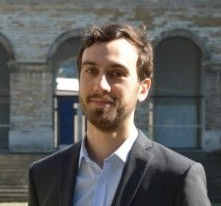
\includegraphics[width=1.2\linewidth]{figs/theo_killian_crop.jpg}
  \end{minipage}
  %&
  \begin{minipage}{.74\textwidth}
    \begin{center}
      % Title 
      \huge \textbf{Exploiting Depmap cancer dependency data using the depmap R package} \\
      \vspace{0.4cm}
      % Authors
      \Large \textbf{Theo Killian, Laurent Gatto} \\
      % Affiliation
      \Large \textit{Computational biology and bioinformatics, de Duve Institute, UCLouvain } \\
      % email
      \vspace{0.4cm}
      \normalsize theodore.killian@uclouvain.be \\
    \end{center}
  \end{minipage}
  %&
  \begin{minipage}{3.7cm}
      
\includegraphics[width=0.7\linewidth, right]{figs/deduve.png} \\
      \vspace{0.5cm}
      
\includegraphics[width=1.1\linewidth, right]{figs/ucl.png}
  \end{minipage}
}
\end{center}


% ---------------------------------------------------------------------------
% Summary

\setlength{\columnsep}{1cm}
\begin{multicols}{2}
\noindent
\fcolorbox{yellow}{yellow}{
  \begin{minipage}[t]{\linewidth}
      \vspace{.15cm}
      \section*{\huge Summary}
      \large The \hcode[yellow]{depmap} package facilitates access in the R environment for data from the \textit{Depmap} project, which maps genetic and chemical dependencies, and other molecular biological features for over 1700 cancer cell lines. The \hcode[yellow]{depmap} package formats this data for use of popular R data analysis and visualization tools such as \hcode[yellow]{dplyr} and \hcode[yellow]{ggplot2}. In addition, the \hcode[yellow]{depmap} package utilizes \hcode[yellow]{ExperimentHub}, storing versions of \textit{Depmap} data accessible from the cloud.
  \end{minipage}
}
\noindent

% ---------------------------------------------------------------------------
% Introduction
\noindent
\begin{minipage}[t]{\linewidth}

  \vspace{-0.50cm}

  \begin{center}
  
\includegraphics[width=0.65\textwidth]{figs/depmap-logo.png}
  \end{center}
   \vspace{-1.25cm}
  % \vspace{0.55cm}
  \section*{\huge Introduction}
  \large Many contemporary cancer drug therapies are broadly toxic to cells. Precision cancer medicine, aims to avoid indescriminate toxicity by exploiting cancer-specific vulnerabilities, termed \textit{dependencies}. However, the exact nature of many of these dependencies in cancer cell lines is not completely understood. The \textit{Depmap} project, a collaboration between the Broad Institute and Wellcome Sanger Institute, maps such dependencies in a broad range cancer cell lines, in the frame of searching for new targets in precision cancer medicine.
\end{minipage}

% ---------------------------------------------------------------------------
% Content of the package
\noindent
\begin{minipage}[t]{\linewidth}
 % \vspace{-2cm}
  \section*{\huge Content of the package}
  \large The \hcode{depmap} package stores all \textit{Depmap} datasets \nocite{meyers2017computational} in the cloud on AWS, via \hcode{ExperimentHub} (\hcode{EH}). \hcode{depmap} accessor functions, such as \hcode{depmap\_rnai()} can be used to retrieve the most current datasets and import them into R. It is also possible to download datasets of specific releases via the \hcode{EH} ID number. \textbf{Help files} with documentation are also provided for every data set.
    \vspace{0.5cm}
    \begin{lstlisting}
  ## automatically download the latest rnai dataset
  rnai <- depmap::depmap_rnai()

  ## or... download specific depmap rnai dataset
  eh <- ExperimentHub()
  query(eh, "depmap")
  rnai <- eh[["EH3080"]]

  ## obtain documentation on depmap rnai dataset
  ?rnai
  \end{lstlisting}
    \vspace{0.5cm}
  \large A table of the available datasets is shown below:
  
  \scriptsize
  \resizebox{\textwidth}{!}{
  \begin{tabular}{@{\extracolsep{15pt}} cl}
  \vspace{0.5cm}
    \\[-1.8ex]\hline
    \hline \\[-1.8ex]
    \textbf{Dataset} & \textbf{Name} \\
    \hline \\[-1.8ex]
    crispr & CRISPR Genetic Dependency (Depmap, Broad 2019) \\
    rnai & RNAi Genetic Dependency (McFarland, et al. 2018) \\
    copyNumber & Gene Level Copy Number (Depmap, Broad 2019) \\
    TPM & TPM Gene Expression (Depmap, Broad 2019) \\
    RPPA & Reverse Phase Protein Array (Ghandi, et al. 2019) \\
    mutationCalls & CCLE Mutation Data (Depmap, Broad 2019) \\
    metadata & Cancer Cell Line Metadata (Depmap, Broad 2019) \\
    drug\_dependency & PRISM Chemical Dependency (Corsello, et al. 2019) \\
    \hline \\[-1.8ex]
    \vspace{0.25cm}
  \end{tabular}}
  
% ---------------------------------------------------------------------------
% Use Cases
  
  \subsection*{\huge Use Case}
  \large
  A potential target in precision cancer medicine is gene \textit{PIK3CA}. Oncogenic mutations of this gene increase dependency on the mRNA cap methyltransferase, \textit{RNMT}, in breast cancer cells. 
  A plot of the dependency scores for all cancer cell lines shows increased genetic dependency for this gene for breast cancer cell lines and that these mutations frequently appear in the COSMIC database. (Figure \ref{fig:dep_table}).  The expression levels of this gene for all cancer cell lines are also illustrated (Figure \ref{fig:exp_table})

\end{minipage}

% ---------------------------------------------------------------------------
% Discussion and Outlook
\vspace{0.4cm}
\noindent
\colorbox{yellow}{
  \begin{minipage}[t]{0.965\linewidth}
    \vspace{0.15cm}
    \section*{\huge Discussion and Outlook}
    \large 
    We hope that this package will serve as a reproducible research framework allowing researchers to easily mine, explore and illustrate dependency data taken from the \textit{Depmap} project. The \hcode{depmap} R package will be maintained in line with biannual \textit{Bioconductor} releases, in addition to incorporating quarterly releases of \textit{Depmap} data. Feedback and questions from the community and contributions to the code are highly appreciated.
  \end{minipage}
}

% ---------------------------------------------------------------------------
% Use Cases
\noindent
\begin{minipage}[t]{\linewidth}
  \vspace{0.55cm}
  \subsection*{}
  % plot 1
  \begin{center}
  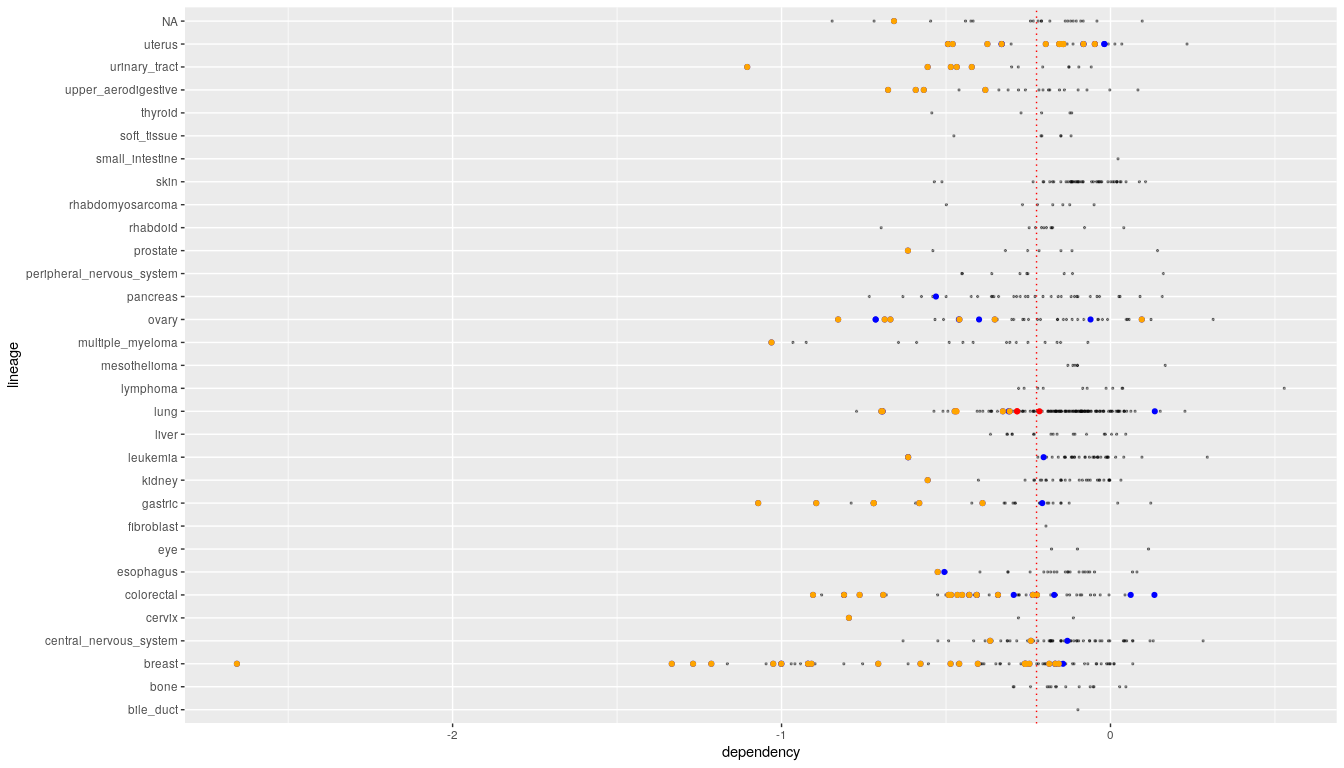
\includegraphics[width=0.95\textwidth]{figs/new_dep.png}
  \end{center}
  \vspace{-0.5cm}
  \captionof{figure}{\textbf{Distribution of RNAi dependency scores for gene PIK3CA by lineage.} \small Types of mutations are highlighted: "damaging" (red), "other non-conserving" (blue), "is COSMIC hotspot" (orange), mean RNAi dependency scores for gene PIK3CA (dotted red line).}
  \label{fig:dep_table}
    \vspace{0.4cm}
  % plot 2
  \begin{center}
  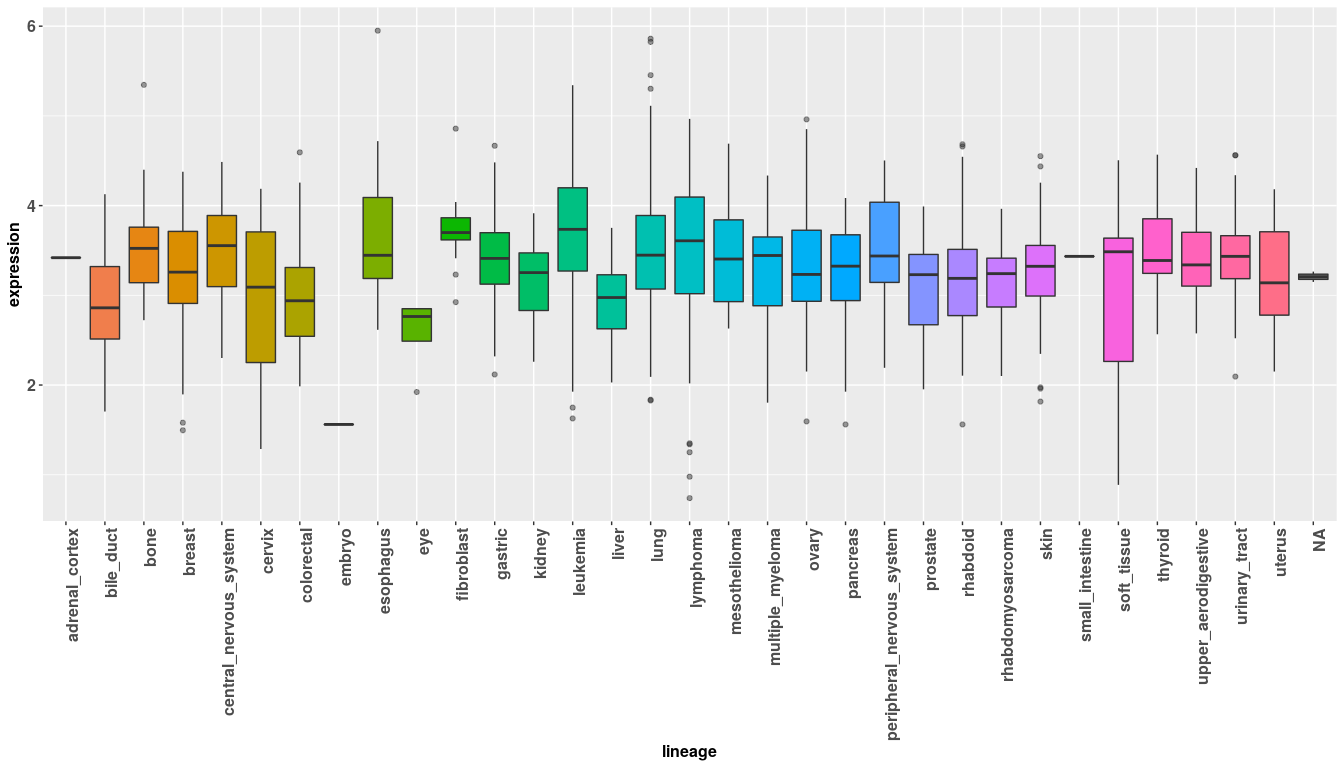
\includegraphics[width=0.95\textwidth]{figs/new_exp.png}
  \end{center}
  \vspace{-0.5cm}
  \captionof{figure}{\textbf{Distribution of gene expression values for gene PIK3CA by lineage.} \small Log2+1 fold expression values for all major cancer diseases. Outliers shown in gray.}
  \label{fig:exp_table}
  %
\nocite{depmap2019depmap}
\nocite{meyers2017computational}
\nocite{mcfarland2018improved}
\nocite{ghandi2019next}
\nocite{li2019landscape}
\nocite{corsello2019non}
\nocite{dempster2019extracting}
\nocite{dunn2019oncogenic}
\nocite{tsherniak2017defining}

% 
% Package Availability
% \noindent
% \begin{minipage}[t]{\linewidth}
\vspace{0.3cm}
  \subsection*{Package Availability}
  \large
  The \hcode{depmap} package is available through \textit{Bioconductor} (since v.3.8) and can be installed in the following manner:
  \begin{lstlisting}
  BiocManager::install("depmap")
  library("depmap")
  \end{lstlisting}
    \vspace{0.3cm}
\end{minipage}

% ---------------------------------------------------------------------------
% References
\scriptsize
\bibliography{references.bib} 
\bibliographystyle{ieeetr}

\end{multicols}

\end{document}